\chapter{Un esempio concreto: il caso MP3}
Per rendere chiara e comprensibile la trattazione sarà portata come esemplificativa uno delle questioni più famose e rilevanti nella storia della brevettazione software, sia per l'importanza dell'invenzione sotto brevetto, sia per la rilevanza economica che ha avuto la causa giudiziaria di violazione di brevetto che ha colpito una delle più importanti aziende informatiche: Microsoft Corporation.

Rilevante sarà anche l'analisi del comportamento che deve essere tenuto nelle varie regioni mondiali in virtù della valenza o meno del suddetto brevetto: per chiarire questa problematica sarà portato come esemplare il comportamento della distribuzione GNU/Linux più diffusa al momento, Ubuntu Linux\cite{ubuntu}.

\section{Cos'è l'algoritmo di compressione MP3}
La discussione di questo capitolo verte su uno degli algoritmi più importanti della storia informatica degli ultimi tempi: l'algoritmo di compressione audio \textit{MPEG-1/2 Audio Layer 3}, comunemente noto come MP3. Questo algoritmo di compressione è diventato noto per la sua capacità di ridurre drasticamente la quantità di dati richiesti per la riproduzione di un suono, mantenendo comunque una riproduzione fedele del suono originario. Nei moderni codificatori MP3 gli algoritmi più efficaci fanno di tutto per assicurare che i suoni rimossi siano quelli che non possono essere rilevati dall'orecchio umano. Questo risultato è stato ottenuto anche grazie alla scienza della psicoacustica.

Nonostante ne siano stati riconosciuti molti difetti, diversi dei quali superati anche da algoritmi successivi ed alternativi (si pensi all'algoritmo \textit{AAC MPEG-4} oppure all'\textit{Ogg Vorbis}) il formato .mp3 (classico dei files compressi con tale algoritmo) risulta ancora il più diffuso in campo musicale, e ciò spiega la portata economica che può comportare l'eventuale copertura brevettuale sull'invenzione.
\section{Il brevetto sull'MP3}\label{mp3-patent}
La Thomson Consumer Electronics è la proprietaria principale del brevetto di MPEG-1/2 Layer 3 in U.S.A. e Giappone, e ha raccolto in un apposito sito (\textit{http://www.mp3licensing.com/}) tutte i brevetti relativi all'MP3 che detiene (svariati validi anche in UE), e una riepilogativa tabella delle royalties che le aziende devono pagare per utilizzare codificatori e decodificatori di MP3.
\begin{figure}[hb]
	\begin{center}
		
\includegraphics[scale=0.75]{figure/mp3.jpg}
	\end{center}
	\caption{\textit{Il logo del sito Thomson sui brevetti MP3}}
\end{figure}
\subsection{Ricerca del brevetto}
almeno una di queste 3 sezioni secondo me andrebbe riempita, magari proprio questa ma è un gran troiaio. alla fine il capitolo è 7 pagine e può andare rimesso in italiano :D però sarebbe meglio...
\subsection{Termini del brevetto}

\subsection{Aree di valenza e royalties}

\section{Il delicato rapporto tra Microsoft ed il formato MP3}
Scendendo nelle notizie di attualità è comune trovare, in campo tecnico/ingegneristico, notizie di violazioni di brevetto, di violazione di proprietà intellettuali e simili. Un po' meno raro è trovare eventi che vedano implicati i brevetti software, specialmente in Europa, dove, come abbiamo visto, sono quasi impossibili da ottenere. 

\`E normale quindi che faccia scalpore quando un tribunale emette una sentenza di violazione di brevetto informatico contro una azienda; è ancora più normale che l'interesse salga a livelli inauditi se l'azienda coinvolta è la più fiorente in campo informatico, e viene condannata ad una pena pecuniaria pari al fatturato di una decina di anni di una azienda normale. Stiamo parlando della Microsoft, e della \textit{querelle} giudiziaria che l'ha vista protagonista con Alcatel-Lucent.

La questione è spinosa in quanto non vede solo motivazioni giuridiche tra i proprietari originari del brevetto ed il presunto violatore, ma vede di fronte al presunto violatore delle enormi aziende che hanno inglobato in percentuali diverse le originali proprietarie del brevetto, lasciando innescare quindi procedure economico/giudiziarie dalla portata enorme.

Nel caso di MP3, come è stato detto nella sezione \ref{mp3-patent}, il principale detentore della proprietà brevettuale è Thomson Consumer Electronics, ma non è affatto ne' l'unica ne' l'originaria proprietaria. Gli algoritmi di base di MP3 sono stati sviluppati originariamente in collaborazione tra il Fraunhofer Institute e gli ex-Bell Laboratories. Il primo gruppo a rilasciare un encoder fu il Fraunhofer Institute nel 1994, e Microsoft ha sempre sostenuto di aver ottenuto in licenza la tecnologia proprio da quest'ultimo, pagandola ben 16 milioni di dollari ed integrandola nei sistemi operativi Windows attraverso i codec e il lettore software Windows Media Player.

Thomson è di fatto la società che al momento controlla il Fraunhofer Institute, mentre Alcatel-Lucent al momento detiene la proprietà dei Bell Laboratories.

Proprio Alcatel-Lucent nel 2003 ha trascinato in tribunale i produttori di PC Dell e Gateway per l'utilizzo illegittimo dei suoi brevetti. Microsoft, in accordo con i patti di indennizzo stretti con le due società, ha offerto loro protezione legale ed ha ottenuto come contropartita la denuncia di Alcatel per la violazione degli accordi di sfruttamento dei brevetti sulla console Xbox 360. Le due aziende avevano stretto un'intesa sulla prima Xbox ma Alcatel-Lucent ha sostenuto davanti al giudice - e ha infine ottenuto una sentenza a proprio favore - che l'accordo non comprendeva la nuova versione; in tutto la disputa riguardava ben quindici violazioni di brevetto, e dopo il rigetto delle prime due accuse, nel Febbraio del 2007 è arrivata la notizia di una sconfitta giuridica per la Microsoft, per la violazione appunto del brevetto riguardante MP3. La sanzione prevedeva una multa per più di un miliardo e mezzo di dollari, valutati i benefici sfruttati abusivamente da Microsoft nel proprio sistema, valutata la diffusione del formato MP3 e la diffusione del sistema Microsoft stesso.

Il motivo principale della diatriba è strettamente legato alle royalties\footnote{Con il termine royalty si indica il pagamento di un compenso al titolare di un brevetto o una proprietà intellettuale, con lo scopo di poter sfruttare quel bene per fini commerciali.} che le aziende devono pagare per poter utilizzare il formato MP3. Come si può vedere nell'elenco pubblico disponibile nel sito Thomson già citato in precedenza, Microsoft risulta considerata tra le aziende autorizzate all'utilizzo della tecnologia; Alcatel, cercando di sfruttare altri processi già aperti contro la casa di Redmond ha tentato di avvalersi del presunto diritto di riscuotere ulteriori royalties sul formato, in virtù dell'acquisizione dei Bell Laboratories.

La questione, ancora non definitivamente sciolta in quanto è ancora possibile un ulteriore grado di giudizio, ha visto la sentenza in appello ribaltare, e di fatto annullare, la sentenza contro Microsoft, riconoscendo sufficiente il pagamento del brevetto presso uno dei proprietari legittimi.

Non ha comunque avuto vita facile la casa di Redmond verso questo formato di compressione audio. Mentre negli Stati Uniti, dove vige il brevetto, ha dovuto sostenere questo lungo processo (non ancora terminato), risulta interessante vedere anche il trattamento che le è stato riservato nell'Unione Europea, dove i brevetti principali dell'MP3 non sono validi.

La Microsoft, dovendo produrre un sistema operativo con bacino d'utenza mondiale, ha inizialmente provato a ``boicottare'' questo formato, cercando di far abituare i suoi utenti al suo formato proprietario (.wma) senza fornire il proprio sistema operativo del supporto per MP3. Questo la lasciava libera negli Stati Uniti dove il brevetto l'avrebbe obbligata al pagamento delle royalties, ma l'ha messa in cattiva luce verso l'Antitrust europeo. 

Il formato .wma a differenza dell'MP3 (che è a specifiche aperte), è a specifiche chiuse e quindi impone all'utente l'utilizzo del software pensato e realizzato dalla stessa Microsoft; d'altro canto la possibilità di essere il produttore del sistema operativo distribuito per più del 90\% sul pianeta aveva indotto la Microsoft a pensare di poter innestare il boicottaggio tramite la procedura di ``abitudine'' degli utenti. 

Sotto la presidenza di Mario Monti, l'antitrust europeo ha comminato alla Microsoft una multa per abuso di posizione dominante con il massimo della sanzione, il 10\% del fatturato. Microsoft è stata costretta ad abilitare l'installazione su Windows di lettori audio diversi dal nativo Windows Media Player, venduto insieme al sistema operativo ad inizialmente l'unico player disponibile sulla piattaforma (e come detto senza il supporto a MP3). Questi software invece dispongono della possibilità di ascoltare l'mp3 e altri formati diversi dal ``.wma'': alla fine, lo stesso software "Windows Media Player" è stato modificato per la lettura di molti codec e la loro masterizzazione, fra i quali c'è l'mp3.

La diatriba tra Microsoft ed il formato MP3 sembra adesso sistemata, in modo positivo per l'azienda negli Stati Uniti ed in modo negativo nell'Unione Europea; la Microsoft resta comunque una delle principali sostenitrici della brevettazione software, intesa come baluardo difensivo del software proprietario e come difesa estrema contro l'avanzata del software libero ed open source. 

Questa presa di posizione sembra quasi confermare la tesi espressa recentemente\footnote{Dal blog personale  http://www.markshuttleworth.com/archives/118} da Mark Shuttleworth, fondatore di Ubuntu, che sostiene quanto non sia la Microsoft stessa la più grossa nemica dello sviluppo open source, ma piuttosto lo sia la possibilità di poter brevettare software in alcuni paesi, che mette moltissime aziende e laboratori di piccole o medie dimensioni in virtù di chiedere royalties pesantissime agli sviluppatori; Microsoft al pari di molte altre aziende e società open source che producono tecnologia (ed anche di più, considerata la distribuzione di Windows), spende cifre sempre più salate per difendersi dalle cause legali relative ai brevetti e per il pagamento delle royalties: questo ha la possibilità di interferire con i piani di sviluppo e rilascio del software, danneggiandola economicamente e portandola con tutta probabilità alla difesa della non brevettabilità del software nel mondo.

Lo stesso Shuttleworth traccia con la propria distribuzione Linux la strada per poter ``convivere'' pacificamente con MP3, senza di fatto pagare royalties o piegarsi a logiche di brevetto.
\section{Il caso Ubuntu: come utilizzare gli MP3 senza violare il brevetto}
Ubuntu è una distribuzione GNU/Linux nata nel 2004 e basata su Debian, che si concentra sulla facilità di installazione e d'uso e sul rilascio regolare (semestrale) delle nuove versioni. 

Finanziata dalla società Canonical Ltd (registrata nell'Isola di Man), rimane comunque in tutto e per tutto un software libero. L'ideatore dell'iniziativa e titolare di Canonical è Mark Shuttleworth, un giovane imprenditore sudafricano diventato fiero sostenitore dell'open source, al cui servizio ha posto le sue risorse.

\`E interessante vedere l'approccio di questa distribuzione sempre nel caso MP3 per due motivazioni distinte: prima di tutto per capire come si sono comportati nei confronti del brevetto vigente ed in seconda battuta per capire come possa il mondo open source sfruttare la loro riuscita nei vari rapporti con software brevettato.

Ubuntu è al momento la principale distribuzione Linux e per questo motivo deve tutelarsi dalla violazione di brevetto, in quanto il suo utilizzo non è vincolato ad una sola zona del mondo ma a tutti i continenti.

In tutte le distribuzioni Linux di \textit{default} è impossibile eseguire un file .mp3; i produttori così si tutelano da eventuali cause contro i detentori del brevetto. Il problema riguarda paesi europei, come l'Italia stessa, dove non c'è vincolo di brevetto per la riproduzione del formato ma ci troviamo comunque di fronte ad un sistema operativo che non lo può riprodurre, vincolato da brevetti stranieri. 

La soluzione pensata da Ubuntu è tanto semplice quanto efficace, e le ha consentito di accaparrarsi solo per questa ragione una discreta fetta di utenza; questa soluzione si basa di fatto sulla responsabilizzazione dell'utenza, e non stravolge di fatto il procedimento da fare nel caso di altre distribuzioni, però lo automatizza.

La prima fase è quella di responsabilizzazione dell'utente; citando direttamente da fonte ufficiale questo è quanto viene comunicato all'utente intenzionato a riprodurre un MP3:``Lo sforzo di Ubuntu nell'includere solo software completamente libero, implica l'esclusione di alcuni formati multimediali proprietari dalla sua installazione. Questa pagina indica i metodi per abilitare il supporto per i formati proprietari più comuni come MP3, WMV e molti altri. Informativa legale: le leggi sui brevetti e sul copyright operano in maniera diversa da paese a paese. Consultare un parere legale se non si è sicuri delle leggi vigenti in materia nel proprio paese.''

A questo punto appare un dialog, simile a quello in figura \ref{dialog}, che richiede all'utente l'abilitazione alla riproduzione del formato MP3. Se l'utente è in un paese come Stati Uniti o Giappone è esclusivamente colpa dell'utente se il brevetto viene infranto, in quanto prima dell'abilitazione è stato correttamente avvisato dei rischi e delle leggi vigenti.

\begin{figure}[htb]
	\begin{center}
		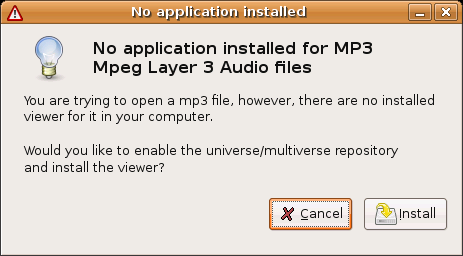
\includegraphics[scale=0.75]{figure/ubuntu_mp3.png}\label{dialog}
	\end{center}
	\caption{\textit{Il primo ``dialog'' per l'installazione del supporto MP3}}
\end{figure}

Questa soluzione, che a livello pratico non richiede particolari competenze informatiche come la capacità di installare il codec MP3 personalmente nel sistema, ha consentito ad Ubuntu di ottenere moltissimi utenti (soprattutto in Europa e negli stati ``liberi'') che non hanno sentito opprimente la copertura brevettuale di altri paesi arrivare fino al proprio.
% \section{Cosa si può fare/non fare in USA in questa circostanza}
% \section{Cosa si può fare/non fare in UE in questa circostanza}
